\documentclass{article}
\usepackage{tikz}
\usetikzlibrary{automata,arrows}

\begin{document}

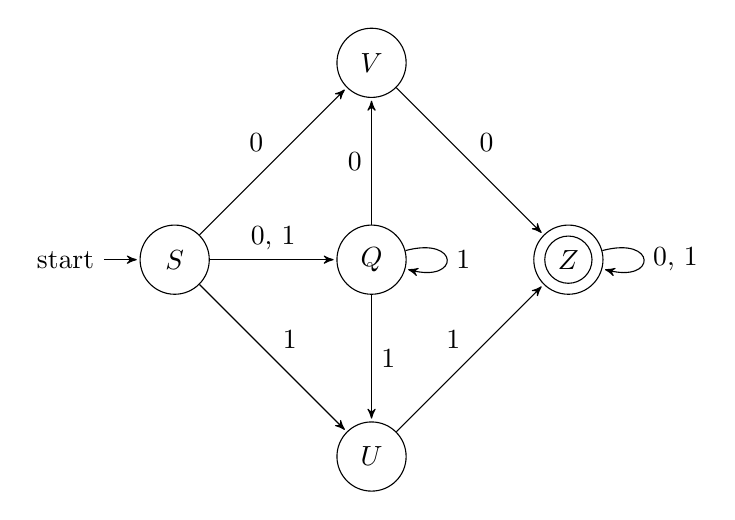
\begin{tikzpicture}[->,>=stealth',shorten >=1pt,auto,node distance=2.5cm]

    % 设置节点(状态)
    \node[state, initial] (S)                {$S$};
    \node[state]           (Q) [right of=S]  {$Q$};
    \node[state]           (U) [below of=Q]  {$U$};
    \node[state]           (V) [above of=Q]  {$V$};
    \node[state]           (Z) [right of=Q]  {$Z$};

    % 画出状态转移的箭头
    % 1. S -> Q, 标签为 0,1
    \draw (S) edge node {0, 1} (Q);

    % 2. S -> U, 标签为 1
    \draw (S) edge node {1} (U);
    \draw (S) edge node {0} (V);
    \draw (U) edge node {1} (Z);
    \draw (V) edge node {0} (Z);

    \draw (Q) edge node {0} (V);
    \draw (Q) edge node {1} (U);

    % 5. Z -> Z, 自环,标签 0,1
    \draw (Q) edge[loop right] node {1} (Q);
    \draw (Z) edge[loop right] node {0, 1} (Z);

    \draw (Z) circle [radius=0.3cm];

\end{tikzpicture}

\vspace{5cm}

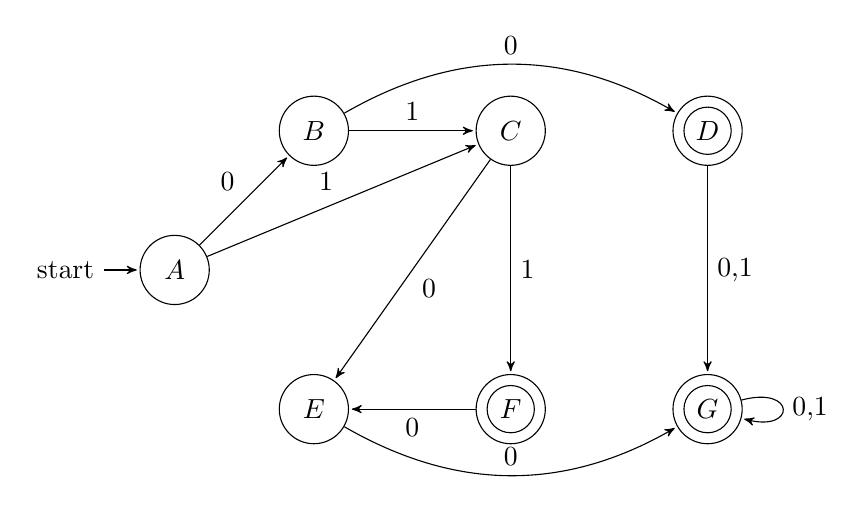
\begin{tikzpicture}[->,>=stealth',shorten >=1pt,auto,node distance=2.5cm]

    % 设置节点(状态)
    \node[state, initial]  (A)                {$A$};
    \node[state]           (B) [above right of=A]  {$B$};
    \node[state]           (C) [right of=B]  {$C$};
    \node[state]           (D) [right of=C]  {$D$};
    \node[state]           (E) [below right of=A]  {$E$};
    \node[state]           (F) [right of=E]  {$F$};
    \node[state]           (G) [right of=F]  {$G$};

    % 画出状态转移的箭头
    % 1. S -> Q, 标签为 0,1
    \draw (A) edge node {0} (B);
    \draw (A) edge node {1} (C);
    \draw (B) edge node {1} (C);

    \draw (B) edge[bend left] node {0} (D);
    \draw (D) edge node {0,1} (G);
    \draw (C) edge node {1} (F);
    \draw (C) edge node {0} (E);
    \draw (E) edge[bend right] node {0} (G);
    \draw (F) edge node {0} (E);

    % % 5. Z -> Z, 自环,标签 0,1
    \draw (G) edge[loop right] node {0,1} (G);

    \draw (G) circle [radius=0.3cm];
    \draw (F) circle [radius=0.3cm];
    \draw (D) circle [radius=0.3cm];

\end{tikzpicture}

\end{document}
